\documentclass[12pt]{elsarticle}
\usepackage{lipsum}
\makeatletter
\def\ps@pprintTitle{%
 \let\@oddhead\@empty
 \let\@evenhead\@empty
 \def\@oddfoot{}%
 \let\@evenfoot\@oddfoot}
\makeatother
\usepackage{graphicx}
\usepackage{pgfplots}
\usepackage{subcaption}
\usepackage{amssymb}
\usepackage{lineno}
\usepackage[margin=1in]{geometry} 
\usepackage{amsmath,amsthm,amssymb}
\begin{document}
\begin{frontmatter}
\title{Face Detection based on Fixed Point Calculations}
\author{Shivang Dave}
\address{University of Houston - Clear Lake}
\begin{abstract}
The primary objective for this research is to find a way to implement one of the integral steps of face recognition - Face detection. In this report, I talk about my implementation of the popular Viola-Jones algorithm \cite{Three}. My implementation emulates all the necessary operations of this algorithm with an alteration. These operations are restructured to adapt fixed point calculations. In addition to this, I release the source code of my implementation to the public domain. I hope that this will allow other researchers to come up with their own results and encourage further research and educational ideas in this area.
\end{abstract}
\end{frontmatter}
\textbf{Source Code:} The source code and demo of this experiment are accessible at the link mentioned at the end of this report\cite{Five}.
\section{Introduction}
\label{S:1}
Face recognition has become significant interest in many applications of intelligent systems such as video surveillance, automotive systems and robotics \cite{Two}. The main challenge of these applications is to recognize objects with an acceptable accuracy while being able to execute it within a few hundred milliseconds on low-cost hardware devices. This research is built upon the idea of performing necessary algorithmic operations over a FPGA board as efficiently as possible. Thus, inspiration of limiting these operations to fixed-point calculations comes from one major drawback of FPGA board(s) that they require more resources to perform floating-point operations. 

\subsection{\textbf{Overview of Viola-Jones Algorithm:}}
\begin{enumerate}
	\item \textit{Input:} 
    \begin{enumerate}
    	\item[] \textit{For training} $\to$ Set of Labeled Images ($x_1$,$y_1$) ... ($x_n$,$y_n$)
    	\item[] \textit{For detection} $\to$ Image(s) ($x_{test}$)
    \end{enumerate}
   	\item Generate Integral Image(s) from input
    \item \textit{Training} $\to$
    \begin{enumerate}
    \item[] For each image in image dataset $\to$ 
        \begin{enumerate}
			\item[-] Apply haar-like features and update weights for each window 
            \item[-] Build a cascade of strong classifiers by combining weak classifiers (Adaboost)
            \item[-] Pass each window through stages to determine probability of finding a face 
            \item[-] If initial stage fails then all other stages will be skipped (Optimization)
        \end{enumerate}
    \end{enumerate}
    \item \textit{Detection} $\to$
    \begin{enumerate}
    	\item[] For each window in the image $\to$
        \begin{enumerate}
			\item[-] Apply cascade of classifiers
			\item[-] If it succeeds in all stages; face detected
        \end{enumerate}
    \end{enumerate}
    \item \textit{End;}
\end{enumerate}

\subsection{\textbf{Background: Detection framework}}

One of the first methods suggested by Paul Viola and Michael Jones in 2001 to provide object detection at very rapid rates \cite{Three}. To increase the detection efficiency adaboost machine learning algorithm is also being used. Main features of the algorithms are: Integral Image, Adaboost and Cascade of classifiers. \\

Integral image is necessary to compute Haar features in a constant time \cite{One}. An integral image can be computed using equation 1. With integration of machine learning, the classification of images becomes much faster as it discards unimportant features from set leaving only the relevant ones. Each feature set is used to create classifiers. 

\[ii(x,y) = {\sum_{x'\leq x,y'\leq y}^{}i(x',y')}\] 
\[s(x,y) = s(x,y-1)+i(x,y)\] 
\[ii(x,y) = ii(x-1,y)+s(x,y)\] 
\[\textit{where s(x,y) = cumulative row sum, s(x,-1) = 0, ii(-1,y)=0} \]
\begin{center}
\textit{Equation 1. Computing Integral Image \cite{Three}} 
\end{center}

Now, these classifiers are applied on each sub-window. But to improve efficiency, a cascade of strong classifiers is used and they are divided into stages. If the window fails in any of the stages then the next following stages are skipped. This can be considered as an optimization parameter. In each stage, Haar-like features of the sub-windows are calculated and compared to the threshold of that stage to see if it contains a face or not \cite{One}. If features satisfies the threshold value only then sub-window advances to the next stage of the cascade. And once it passes all the stages then the sub-window is labeled as positive detection.\\

An optimal algorithm is required to work with reasonable resources. Techniques such as integral image and attentional cascade make the Viola-Jones algorithm \cite{Three} highly efficient. Using OpenCV's precomputed haar cascade classifier (frontal face) for building face detection system allows very fast execution of the algorithm.

\section{Implementation}
\label{S:2}

The proposed implementation mainly focuses on face detection by performing essential operations in fixed-point manner. To accomplish this task, we needed to make sure that each operation and all the values involved in such operations are bounded to a fixed point by certain precision. Python's \textit{decimal} library enabled conversion of floating point values to fixed-point with a certain precision.\\

Initially, an image is provided to the program. Once that image loads successfully, pixel density matrices are created. These matrices are then used to generate integral image of the input image. In addition to the integral image, we are training a haar cascade classifier by parsing pre-compiled list of stages from OpenCV's frontal face feature set. As soon as the classifier finishes parsing, a 20x20 sub-window is generated. This sub-window performs classification by calculating and comparing threshold values for each stage. This way it is able to evaluate if that window contains a face or not. 

\subsection{\textbf{Pseudo-code for implementation:}}
\begin{enumerate}
	\item \textit{Input: Test Image}
    \item \textit{Output: Image with rectangle drawn around face if detected}
   	\item Generate Integral Image from input image
    \item \textit{Detection:}
    \begin{enumerate}
    	\item[] For each sub-window in the image $\to$
        \begin{enumerate}
			\item[] Apply cascade of classifiers
            \begin{enumerate}
				\item[] Feature detection in sub-window
				\item[] If feature\_sum doesn't match threshold $\to$
                		 \subitem Reject sub-window
                \item[] Else:
                		 \subitem Move to next stage
        	\end{enumerate}
			\item[] If sub-window passes all stages:
            		\subitem Accept it as a face
        \end{enumerate}
        \item[] Draw a rectangle
    \end{enumerate}
    \item \textit{Exit;}
\end{enumerate}

If the sub-window is able to validate through all the essential stage thresholds, then it is classified as a facial image. Whenever a sub-window passes stage evaluation, its position is stored in an array. This array should contain redundant values as the sub-window size is very small compared to input image. Hence, array is then cleaned to get rid of those redundant results after classification is complete. After cleaning the array it becomes easier to annotate the face by drawing a rectangle around it. Output is shown in Figure 2.

\subsection{\textbf{Dependencies:}}
\begin{enumerate}
\item[-] Language: Python 2.7
\item[-] Library: PIL (used for image processing)
\item[-] Library: lxml (used for parsing haar features from OpenCV's XML file)
\item[-] Library: Decimal (used for converting data points to fixed points)
\item[-] Detector: Haar cascade frontal face by OpenCV (used for trained classifier)
\end{enumerate}

\textit{Note: Decimal library is used to bound floating point values to decimal fixed-point representation. Each arithmetic operation such as division, square, square roots etc are bounded to fixed-point calculations.} 

\subsection{\textbf{How to run:}}
\begin{enumerate}
\item[-] Move to the project directory in terminal and type following:
\begin{center}
\subitem \textit{python exec.py}
\end{center}
\item[] Options:
\item[] Execute it for all the images in \textit{img} folder:
\begin{center}
\subitem \textit{python exec.py}
\end{center}
\item[] Execute it for a specific image in \textit{img} folder:
\begin{center}
\subitem \textit{python exec.py 1.jpg}
\end{center}
\item[-] Hit enter!
\end{enumerate}

\begin{figure}[ht]
\centering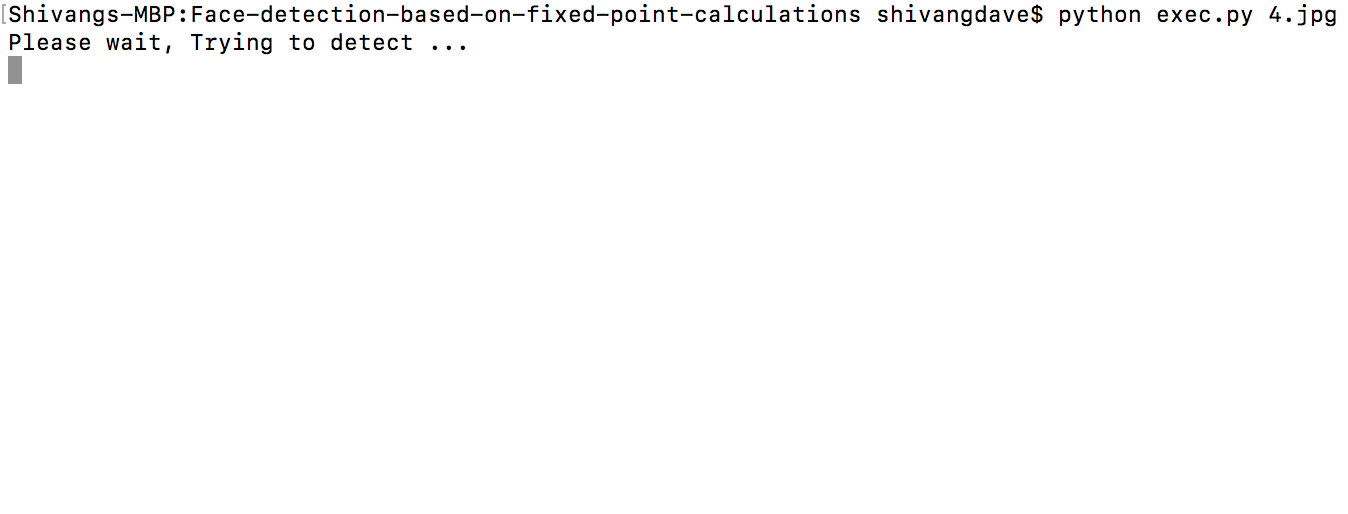
\includegraphics[width=0.7\linewidth]{input_cmd.png}
\caption{Input for single image}
\end{figure}

\section{Results:}
\label{S:3}

\begin{figure}
\begin{subfigure}[ht]{0.5\linewidth}
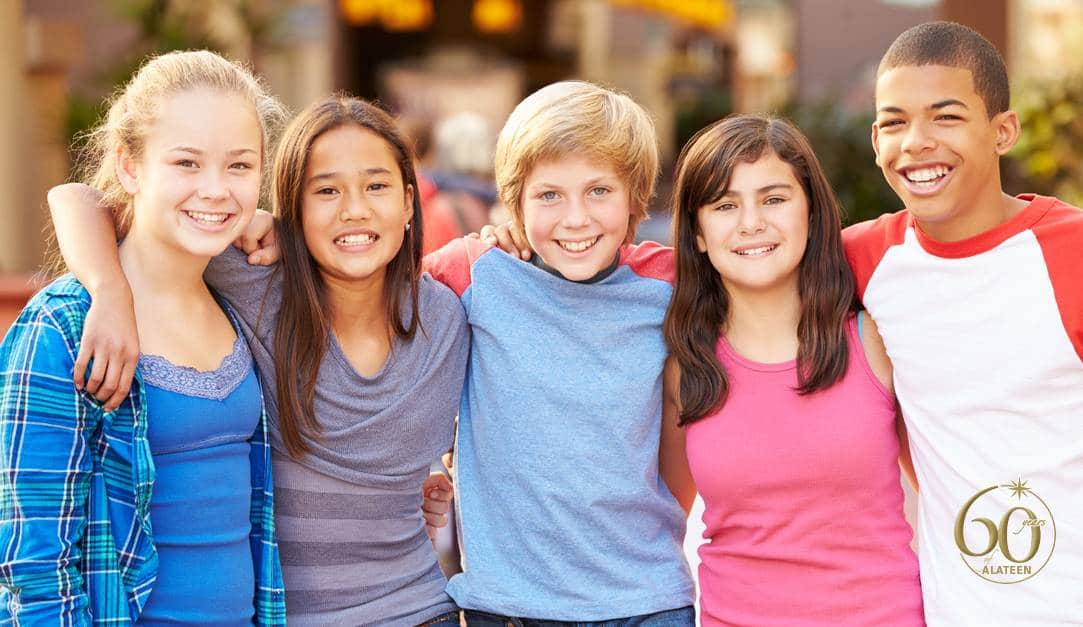
\includegraphics[width=\linewidth]{input.jpg}
\caption{Input Image}
\end{subfigure}
\hfill
\begin{subfigure}[ht]{0.5\linewidth}
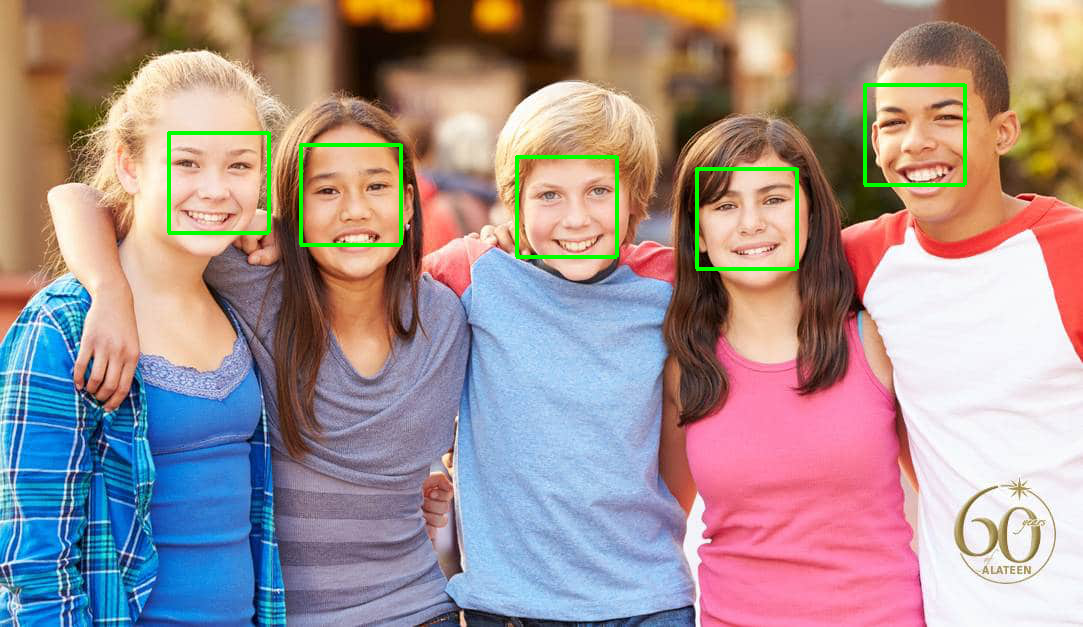
\includegraphics[width=\linewidth]{output.png}
\caption{Output Image}
\end{subfigure}%
\caption{Output}
\end{figure}

As expected due to increase in number of operations, time complexity suffers a lot. As we can see in Table 1, Fixed-point operations take almost 8x the time floating-point operations take on same image with similar detection accuracy. We can reduce the time complexity by giving up the detection accuracy. So, it proves the trade-off between time complexity and detection accuracy.\\

\begin{table}[h!]
\centering
\begin{tabular}{||c|c|c||} 
 \hline
 Image & Fixed-point & Floating-point \\ [0.5ex] 
 \hline\hline
 1.jpg & 8.57 & 1.38  \\ 
 2.jpg & 28.0 & 3.73  \\
 3.jpg & 10.58 & 1.67 \\
 4.jpg & 35.60 & 4.30 \\
 5.jpg & 23.18 & 3.10 \\ [1ex] 
 \hline
\end{tabular}
\caption{Execution time (in seconds)}
\label{table:1}
\end{table}

As we can see in Graph 2, Increased window scaling deteriorates detection accuracy but improves execution time significantly. Thus, in the end to decide whether to improve accuracy or improve time complexity will depend on the type of application and its use cases.

\section{Conclusion:}
\label{S:4}
Viola-Jones Algorithm \cite{Three} introduced an approach for object detection which minimized computation time while achieving high detection accuracy. But along with the high accuracy it required resource hungry computations. With my implementation, I have tried simplify these computations by bounding them to a certain fixed-point. This implementation can be used as a reference to design different applications for many resource restricted platforms such as FPGA boards, IoT devices and more. I hope that this detailed report will enable easy replications and comparison of results. And more importantly, will encourage further research.

\begin{center}
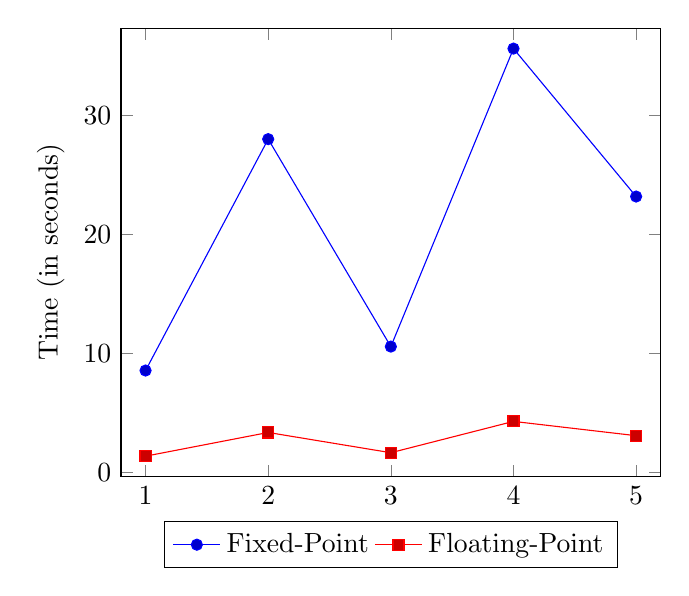
\begin{tikzpicture}
\begin{axis}[
	x tick label style={
		/pgf/number format/1000 sep=},
	ylabel=Time (in seconds),
	enlargelimits=0.05,
	legend style={at={(0.5,-0.1)},
	anchor=north,legend columns=-1},
]
\addplot 
	coordinates {(1,8.57) (2,28.0)
		 (3,10.58) (4,35.60) (5,23.18)};
\addplot 
	coordinates {(1,1.38) (2,3.37)
		 (3,1.67) (4,4.30) (5,3.10)};
\legend{Fixed-Point,Floating-Point}
\end{axis}
\end{tikzpicture}
\\Graph 1: Execution Time
\end{center}

\begin{center}
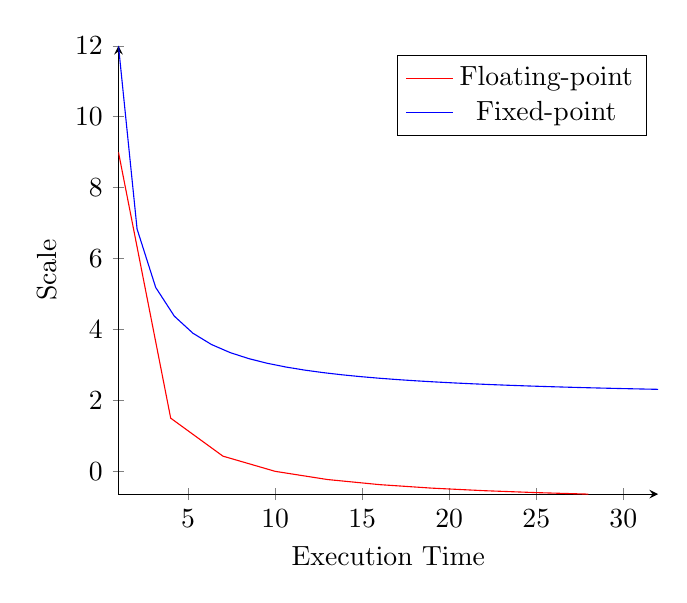
\begin{tikzpicture}
\begin{axis}[
    axis lines = left,
    xlabel = Execution Time,
    ylabel = Scale,
]
\addplot [
    domain=1:28, 
    samples=10, 
    color=red,
]
{10/x-1};
\addlegendentry{Floating-point}
\addplot [
    domain=1:32, 
    samples=30, 
    color=blue,
    ]
 {10/x+2};
\addlegendentry{Fixed-point}
 
\end{axis}
\end{tikzpicture}
\\Graph 2: Scale vs Execution Time
\end{center}

\section{Image Credits:}
\label{S:5}
\begin{enumerate}
\item Google Image Search.
\item OpenCV.
\item The USC-SIPI$^7$ Image Database.
\end{enumerate}

\section{Instructors:}
\label{S:6}
\begin{enumerate}
\item Dr. Xiaokun Yang, UHCL
\item Dr. Kewai Sha, UHCL
\end{enumerate}

\section{References:}
\label{S:7}
\begin{thebibliography}{999}

	\bibitem{One}
	  Abdul Mohsen Abdul Hossen, Raheem Abd Alsaheb Ogla, Maitham Mahmood Ali, Face Detection using OpenCV's Viola-Jones Algorithm based on coding eyes
  	  \emph{University of Technology, Baghdad, Iraq}.
  	  Iraqi Journal of Science,
	  Vol. 58, No.2A,
  	  2017.
      
  	\bibitem{Two}
	  Imran Naseem, Roberto Togneri, Mohammed Bennamoun, Linear regression for Face Detection
  	  \emph{Senior Member, IEEE}.
  	  IEEE Transactions on Pattern Analysis and Machine Intelligence,
	  Vol. 32, Issue: 11,
  	  Nov. 2010.
      
    \bibitem{Three} 
	  Jones, M. and Viola, P., Rapid Object Detection using a Boosted Cascade of Simple Features.
  	  \emph{Senior Member, IEEE}.
  	  Computer Vision and Pattern Recognition. IEEE Computer Society Conference,
  	  2001.
      
     \bibitem{Four} 
	  Yi-Qing Wang, An analysis of the Viola-Jones Face Detection Algorithm
  	  \emph{CMLA, France}.
  	  Published in Image Processing On line. ISSN 2105-1232,
  	  2014.
      
     \bibitem{Five} 
	  Shivang Dave, Face detection based on fixed-point calculations
  	  \emph{University of Houston - Clear Lake}
  	  2018.
      Source Code: https://github.com/ShivangDave/Face-detection-based-on-fixed-point-calculations
      
\end{thebibliography}

\end{document}